

% Chapter 2

\chapter{Background}
\label{chap:background} 

Programming in strongly typed languages has many advantages. It helps programmers identify logical errors before running the code, reduce maintenance difficulty, and improve the editor capability find documents and auto-complete code while typing. However, the difficulties in understanding and resolving type errors often ward people off  from practicing strongly typing.  In this Chapter, we discuss the relevant research in improving the experience of debugging type errors. We first investigate the theoretical approaches to enrich/correct the information presented type errors. We then  investigate the various designs of tools, interfaces, and visualizations to support understanding type errors.

\graphicspath{{Figures/Background}}




\section{Functional Programming}

Functional programming is a programming paradigm that treats computation as the evaluation of mathematical functions and avoids changing state and mutable data. The roots of functional programming are deeply embedded in mathematics, stemming from the lambda calculus - a mathematical system built around function abstraction and application - developed by Alonzo Church in the 1930s.


The early functional programming languages include Common Lisp in the 1950s, Scheme invented in the 1970s, and ML in the 1970s. In the 80s  the language Miranda was developed, introducing the world to more flexible functional concepts, such as lazy evaluation. However, some of these ideas were commercialised, which spurred the creation of Haskell – a purely functional language produced by the open-source community, later becoming a seminal achievement and most influential functional language in academia and the programming industry.


In the 21st century, although new functional programming languages are continue to be created, such as Clojure, F*, and Idris, what’s more often interesting to see is functional programming ideas and benefits into other paradigms. Scala is a programming language that combines the expressiveness of functional composition and ergonomics of object oriented programming. JavaScript, a traditional multi-paradigm language, started to adopt programming features such as lexical scoping, tail recursion optimization.


In 1978 John Backus delivered his Turing Award lecture, “Can programming be liberated from the von Neumann style?”, bringing functional programming into the recognition in the larger programming world. Different from other paradigms in the programming realm, functional programming brought a few innovations that changed the thinking in the academic and programming community, and has been sought after by other paradigms for decades to come.


\textbf{Declarative}: being close to mathematical functions, functional programs are the composition of forms that map value from one domain to another. Instead of explaining how to achieve a specific task step-by-step (like in imperative languages), functional programming encourages developers to describe what they want to achieve and the language abstracts the how.


\textbf{Immutability}: Unlike object-oriented programming, where data structures (such as objects) could be changed, or mutated, data in functional programming is immutable, meaning it cannot be changed after creation. This trait reduces the chances of bugs because you know that your data isn't changing unexpectedly.


\textbf{Pureness}: pure functions are functions that observe referential transparency, in other words when given the same input will always reach the same output. The pureness of functional programming seems to be a big restriction and handicap on what a function can do, for instance, that pure functions cannot access external systems or produce true random numbers. However, pure functions are as potent as they are limiting, it creates a strong separation between data and programs and powerful transformation can be developed on the premise that no side effects are present in the programs.


\textbf{High order functions}: The idea of using functions as normal values where they can be assigned to names, returned by other functions, or passed as arguments is a fundamental ingredient of functional thinking. This aspect allows programmers to create more abstract functions and reusable logic. Currying is a special case of high order function, where a function with multiple arguments is transformed into a sequence of functions, each with a single argument. Currying is beneficial for creating simpler and cleaner functions and aids in code reusability.

\section{Statically Typed Languages and The Typing Debate}


Static typing has been practised since the very start of programming languages. Fortran, known as the first compiled programming language, has explicit types for integers and floating point numbers, and uses static typing to reject mal-formed programs. Later programming languages Pascal, C were all designed to use static typing. In these languages, user defined types, such as functions and structs, have become available, making the type checking more flexible and reliable.

 
Functional languages, especially Haskell, took the static types further with ideas coming from academic languages, such as typed lambda calculus and system F, that are shown to be sound and complete. Many type-level features in Haskell were later exported to languages of other paradigms.  Polymorphic types were introduced to allow functions types to be defined more fluidly so that they can work with any data types. Type inference (also known as implicit types) was introduced to allow static type checking even without any explicit type annotations. These features can now be found in most mainstream programming languages. (Give an examples of )


Compared to static typing, the alternative typing discipline – dynamic typing – provides many appealing benefits, and has strong influence in the computing world. In dynamically typed languages, a variable can hold different types of values because the type is checked during runtime. This provides more flexibility than static typing since a single variable can be used to hold different types of values through mutation or reassignment. However, it also means that errors such as trying to subtract a string from a number can be detected only when the code is run, leading to potential runtime errors.


The lisp programming languages, such as common lisp and scheme, were designed to benefit from the flexibility of dynamic typing. In Lisp languages, functions often take dynamic input that can be various forms (atom, lists, s-expressions), and different code is executed based on inspecting the input value at runtime. In modern day computing,  languages like JavasScript, Python are all dynamic languages, which is believed to contribute to their immense popularity thanks to the lower barrier of entry.

\subsection{The arguments for static typing}
\textbf{Program safety}: Static typing can catch errors and bugs during compile time, before the software even runs. This can be particularly beneficial when working on large code bases or complex systems.

\textbf{Ease of Maintenance}: Static typing allows common software engineering tasks, such as refactoring code more reliable. In general, a software project will not successfully compile unless all the  locations affected by the initial changes are addressed and resolved.

\textbf{Additional Tooling Support}: The type information in static languages can help programmers understand code better and faster. This is often shown as richer information in documentation, or more detailed pop-over type hints with modern programming IDEs.  

\subsection{The arguments for Dynamic typing}

\textbf{Ease of Use and Flexibility}: Dynamically typed languages usually have a simpler syntax, and the flexibility of being able to change the type of a variable on the fly.

\textbf{Rapid Prototyping}: Dynamic typing can be faster in terms of development, facilitating quick prototyping and scripting.

\textbf{Metaprogramming}: Dynamically typed languages are robust in metaprogramming because they can inspect, generate, and modify code more flexibly during runtime.


\section{The Mission To Improving Type Errors}


Type errors can be notoriously difficult to understand and use, particularly for newcomers to programming or when using a language that is more strict about types. Type errors are often believed to be a major contributor to static typing's popularity. Type errors can happen in dynamic languages as well, however, they are not as difficult as their counterparts in static languages.


To start, the languages used in deceiving type errors are unhelpful to programmers. On one side, type errors often involve terminology and concepts that can be difficult to understand, particularly for less experienced programmers. The concepts might include objects, instances, classes, functions, variables, or aspects of data types that haven't been encountered before or fully understood. This is exemplified to extremes in Haskell, where programmers are often perplexed by errors like “No instance for (Num Char) arising from the literal '1'”. One another side,  the error messages returned for type errors are either vague or misleading. They might indicate the line of code where the error was detected but the actual mistake might be somewhere else.


Another factor of the difficulty of type errors is the lack of supporting information. Programmers can get stuck in a type error for hours and concede that dynamic languages are easier. When type errors are at runtime, programmers can at least run the program and insert printing statements to observe the dataflow of the program. None of these debugging techniques work on type errors as they are reported without actually running the program.  This is  comparable to debugging parse errors, which also happen at compile time. But generally parse errors are often local, meaning that a parse error has a sensible range of locations,  indentation errors can be searched in the parent indentation block, unmatched brackets can be searched in the outermost brackets. On the other hand, type errors are more global, a type conflict can happen between two different files, or code from different sources. This added to the difficulties of solving type errors.
 

Type errors are made harder with more advanced type system features have been introduced. As a result the usability of type systems decreases as the expressiveness of the type system increases. For example polymorphic types allow types to be defined to restrict the relations between types instead of the types themselves. For example the (==) :: a -> a -> Bool function can be defined to compare two values of the same type, without specifying which type it must be. However, this will add confusion when too many polymorphic variables are participating in the type error and compilers sometimes rename them to further mystify the case.


Throughout history, many have dedicated their research to improving type errors, making them easier to understand and better at helping to find the root causes. We categorise them into three major themes: Enhanced compiler error message, reporting multiple nodes, and interactive debugging.

\subsection{Enhanced Compiler Error Messages}

A well-studied approach to producing better error explanations is through ECEM (Enhanced compiler error message).  As put in~\cite{Barik2017-gy}, ``Error messages appear to take the form of natural language, yet are as difficult to read as source code."   Through a series of mixed-method studies, Prather showed~\cite{Prather2017-dg} that ECEM has a positive result in understanding compiler errors. Decaf~\cite{Becker2016-kc} is a tool that can rephrase Java compiler error messages into an enhanced version. In a study of over 200 CS1 students, Decaf was shown to reduce overall errors in their coding practices. Berik proposed a framework~\cite{Barik2018-xs} for constructing compiler error messages based on argumentation theory, and showed that error messages following a simple argumentation layout or an extended argumentation layout are more human-friendly.  These works show the significance of improving the language in the compiler error messages. 


\subsection{Reporting Multiple Nodes}

\begin{figure}[hbt]
    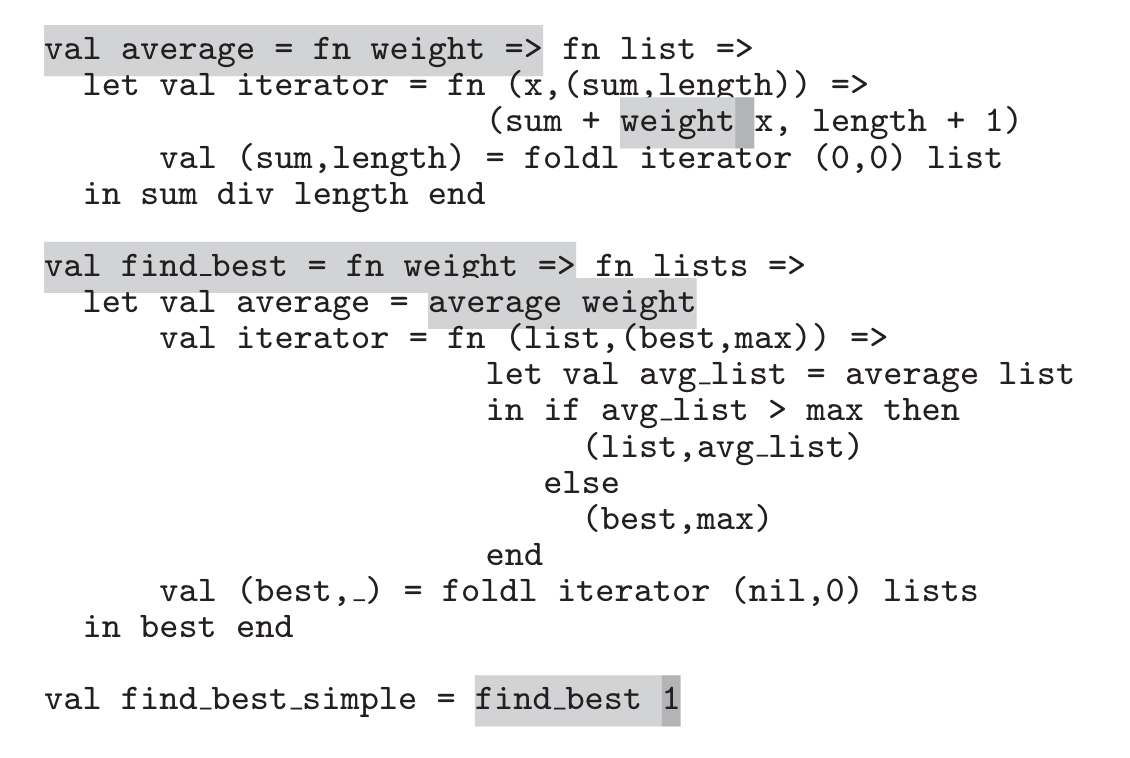
\includegraphics[width=0.6\linewidth]{HaackTypeErrorSlicing}
    \caption{An example of Type Error Slicing by Haack and Wells
    }
\end{figure}

Many have studied the approach of finding all locations that contribute to a type error~\cite{Stuckey2003-pz, Haack2004-fr, Pavlinovic2015-ke, Schilling2012-iq}. Type error slicing~\cite{Haack2004-fr} is a technique that finds locations that are complete and minimal for the type error. Internally labeled constraints and Minimal Unsatisfiable Subset (MUS) generation are used to generate these slices. The language supported in Haack's work was a subset of Standard ML. The original Chameleon~\cite{Stuckey2003-pz} used  Constraint handling rules (CHR) to support the computing of type error slices in Haskell. Chameleon also supported advanced type-level features (type classes and functionally dependent types). The project also introduced the ability to query type information through a command line interface. Although Chameleon was firmly grounded in results from type theory, its designs were never evaluated with user studies. While finding all error locations is useful in comprehending type errors, it is only 1 of the 7 properties listed in the proposed manifesto of good type error reporting~\cite{Yang2000-wn}.

\subsection{Interactive Debugging}

\begin{figure}[hbt]
    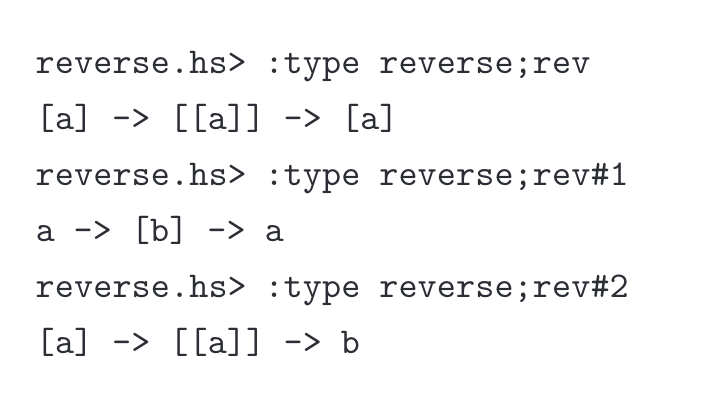
\includegraphics[width=0.6\linewidth]{ChameleonInteractive}
    \caption{An example of Type Error Slicing by Haack and Wells
    }
\end{figure}
Interactive debugging is a method in which programmers can selectively view the debugging information, test and retract their assumptions, and  make changes and observe their effects. Interactive debuggings have been practised for a long time for debugging runtime errors. Programmers often use techniques such as pause/break (also known as a breakpoint) a running program, inspect the current state, and change values if needed. It's highly beneficial because it allows the programmer to interact with the program at runtime, which can provide valuable insights into the state of the program and help identify errors. However, for type errors, programmers are stuck with static error messages in text form. However some early ideas of interactive debugging were proposed in research. Chameleon is an Haskell interactive type debugger that works in command line interface. When encountering a type error, Chameleon is able to analyse and deduce alternative ways a type error can be fixed, and programers can select an alternative they desire by typing in command.


\section{Verify Generated Source Code -- a case for the future}

One trend we have seen in recent years is that generative AI models are widely used to generate code. Once trained, these models can generate code snippets or complete applications based on user input. This might take the form of a natural language prompt, a framework or blueprint layout of the needed application, or even a sequence of tasks or features the code is intended to address. Many models trained in large corpus of software projects show competence in producing source code according to human prompts. However, it seems inevitable that source code generated by a large language model may contain errors, undesired behaviours, or even critical security vulnerabilities. Another big concern is that it is hard to get a grip of the accuracy of AI generated code with popular metrics. In this, human evaluation is still significantly better than automated metrics.


 We believe that statically typed functional languages are the ideal candidates for code generations of these tools. The functional requirements force the pure functions and effect to be clearly separated, where undesired behaviours, such as making database connections, or sending network packets to an external party, are harder to sneak in. In addition, the static typing forces that the generated code must be conformative to the specification. And thus, we strongly believe that now more than ever, we need intuitive type error messages, and streamlined type error debugging processes, to accommodate traditional human written programs, and to tame the AI generated code.


 \section{Conclusion}
 In this chapter, we followed the footsteps of the historical development of functional programming languages and statically typed languages, and their current status in academia and the programming industry. We showed through multiple studies where there is a lack of attention in the design of type errors. We explored multiple research projects that were dedicated to improving the type errors and the way programmers debugging them. We also took a peek at the potential future of programming, and how our effort in improving type errors may help brighten such a future.